\documentclass[a4paper]{scrreprt}

\usepackage{scrhack}
\usepackage{graphicx}
\usepackage[utf8]{inputenc}

\addtokomafont{titlehead}{\flushright}
\addtokomafont{subject}{\vspace{3cm}\flushleft}
\addtokomafont{title}{\flushleft}
\addtokomafont{subtitle}{\flushleft}
\addtokomafont{author}{\flushleft\setlength{\tabcolsep}{0pt}}
\addtokomafont{date}{\flushleft}
\addtokomafont{publishers}{\flushleft}

\titlehead{
\includegraphics[scale=2]{../templates/logo_en}}
\subject{Software Engineering and Design}
\title{Document Title}
\subtitle{Mental Health Care Patient Management System (MHC-PMS)}
\author{
\begin{tabular}{l}
\normalfont\bfseries{Team White:}\\
Dellsperger Jan\\
Ellenberger Roger\\
Sheppard David\\
Sidler Matthias\\
Spring Mathias\\
Thöni Stefan
\end{tabular}
}
\date{\today}
\publishers{Version 1.0}

\begin{document}

\begin{titlepage}
	\maketitle
\end{titlepage}

\chapter{UML Domain Model}

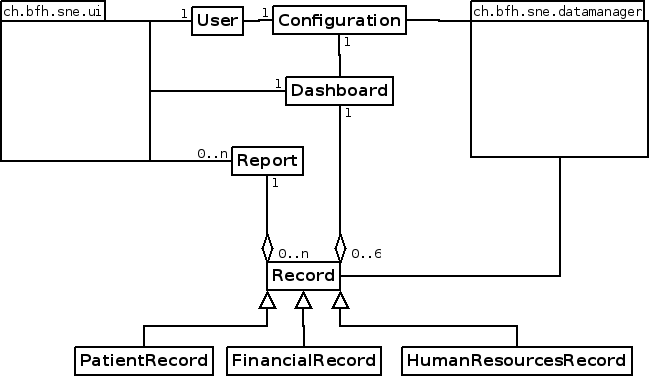
\includegraphics[width=1\textwidth]{./class-diagram.png}

\paragraph{User} ist die Klasse, welche die Authentifizierung des Benutzers realisiert. Zudem sind  Daten über den Benutzer in dieser Klasse abgebildet.

\paragraph{Configuration} als Klasse beinhaltet die benutzerspezifische Konfiguration der Applikation. Dies sind hauptsächlich Dashboard-Konfigurationen. Diese Daten werden serverseitig gespeichert, damit diese Geräte-Unabhägig überall gleich sind - egal ob der Benutzer mit seinem Tablet, seinem Smartphone oder seiner Workstation auf die Applikation zugreift.

\paragraph{Dashboard} bildet die logische Komponente des Dashboards ab, welches auch ein zentraler Bestandteil des GUI's ist. Das Dashboard ist an sich unabhängig vom Dashboard. Lediglich über die Grafische Oberfläche haben sich die beiden Klassen eine gewisse Abhängigkeit. Die ist aber in der Programm-Logik nicht nötig.

\paragraph{Report} ist die Klasse, welche die Auswertungen der Daten ausführt. Daher besteht eine Abhängigkeit zur Klasse Record. Ein Report kann auf mehrere Datenrecords zugreifen um seine Auswertungen bereitzustellen.

\paragraph{Record} Beinhaltet die Daten, welche der Datamanager der Applikation bereitstellt. Record ist zudem Superklasse von \textbf{PatientRecord}, \textbf{FinancialRecord} und \textbf{HumanResourcesRecord}, welche die verschiedenen Ausprägungen der vorhanden Daten abbilden.

\paragraph{ch.bfh.sne.ui} ist das zuständige Package für die Grafische Oberfläche.

\paragraph{ch.bfh.sne.datamanager} ist das zuständige Package, welches die Schnittstelle zwischen Datenbank und Applikation realisiert.


\section{Name}
Damit wir bereits realitätsnahe Package-Namen definieren konnten, haben wir für unsere Applikation einen Namen gesucht. Dabei fanden wir gefallen an einem rekursiven Akronym, welches aus unserer Sicht sehr passend ist zu unserem Projekt.

\begin{quote}
SNE: \textbf{S}NE is \textbf{n}ot \textbf{E}-Health
\end{quote}

Wir sehen uns nicht als Teil von E-Health, da wir moderner sind als dieser Trend.


\chapter{UML Sequence Diagram}

\section{Benutzer aktualisiert Informationen}
Der Benutzer verfügt nicht über die Möglichkeit Datensätze zu verändern. Eine der wenigen Daten die der Benutzer verändern kann, ist seine Dashboard-Konfiguration.

\bigskip

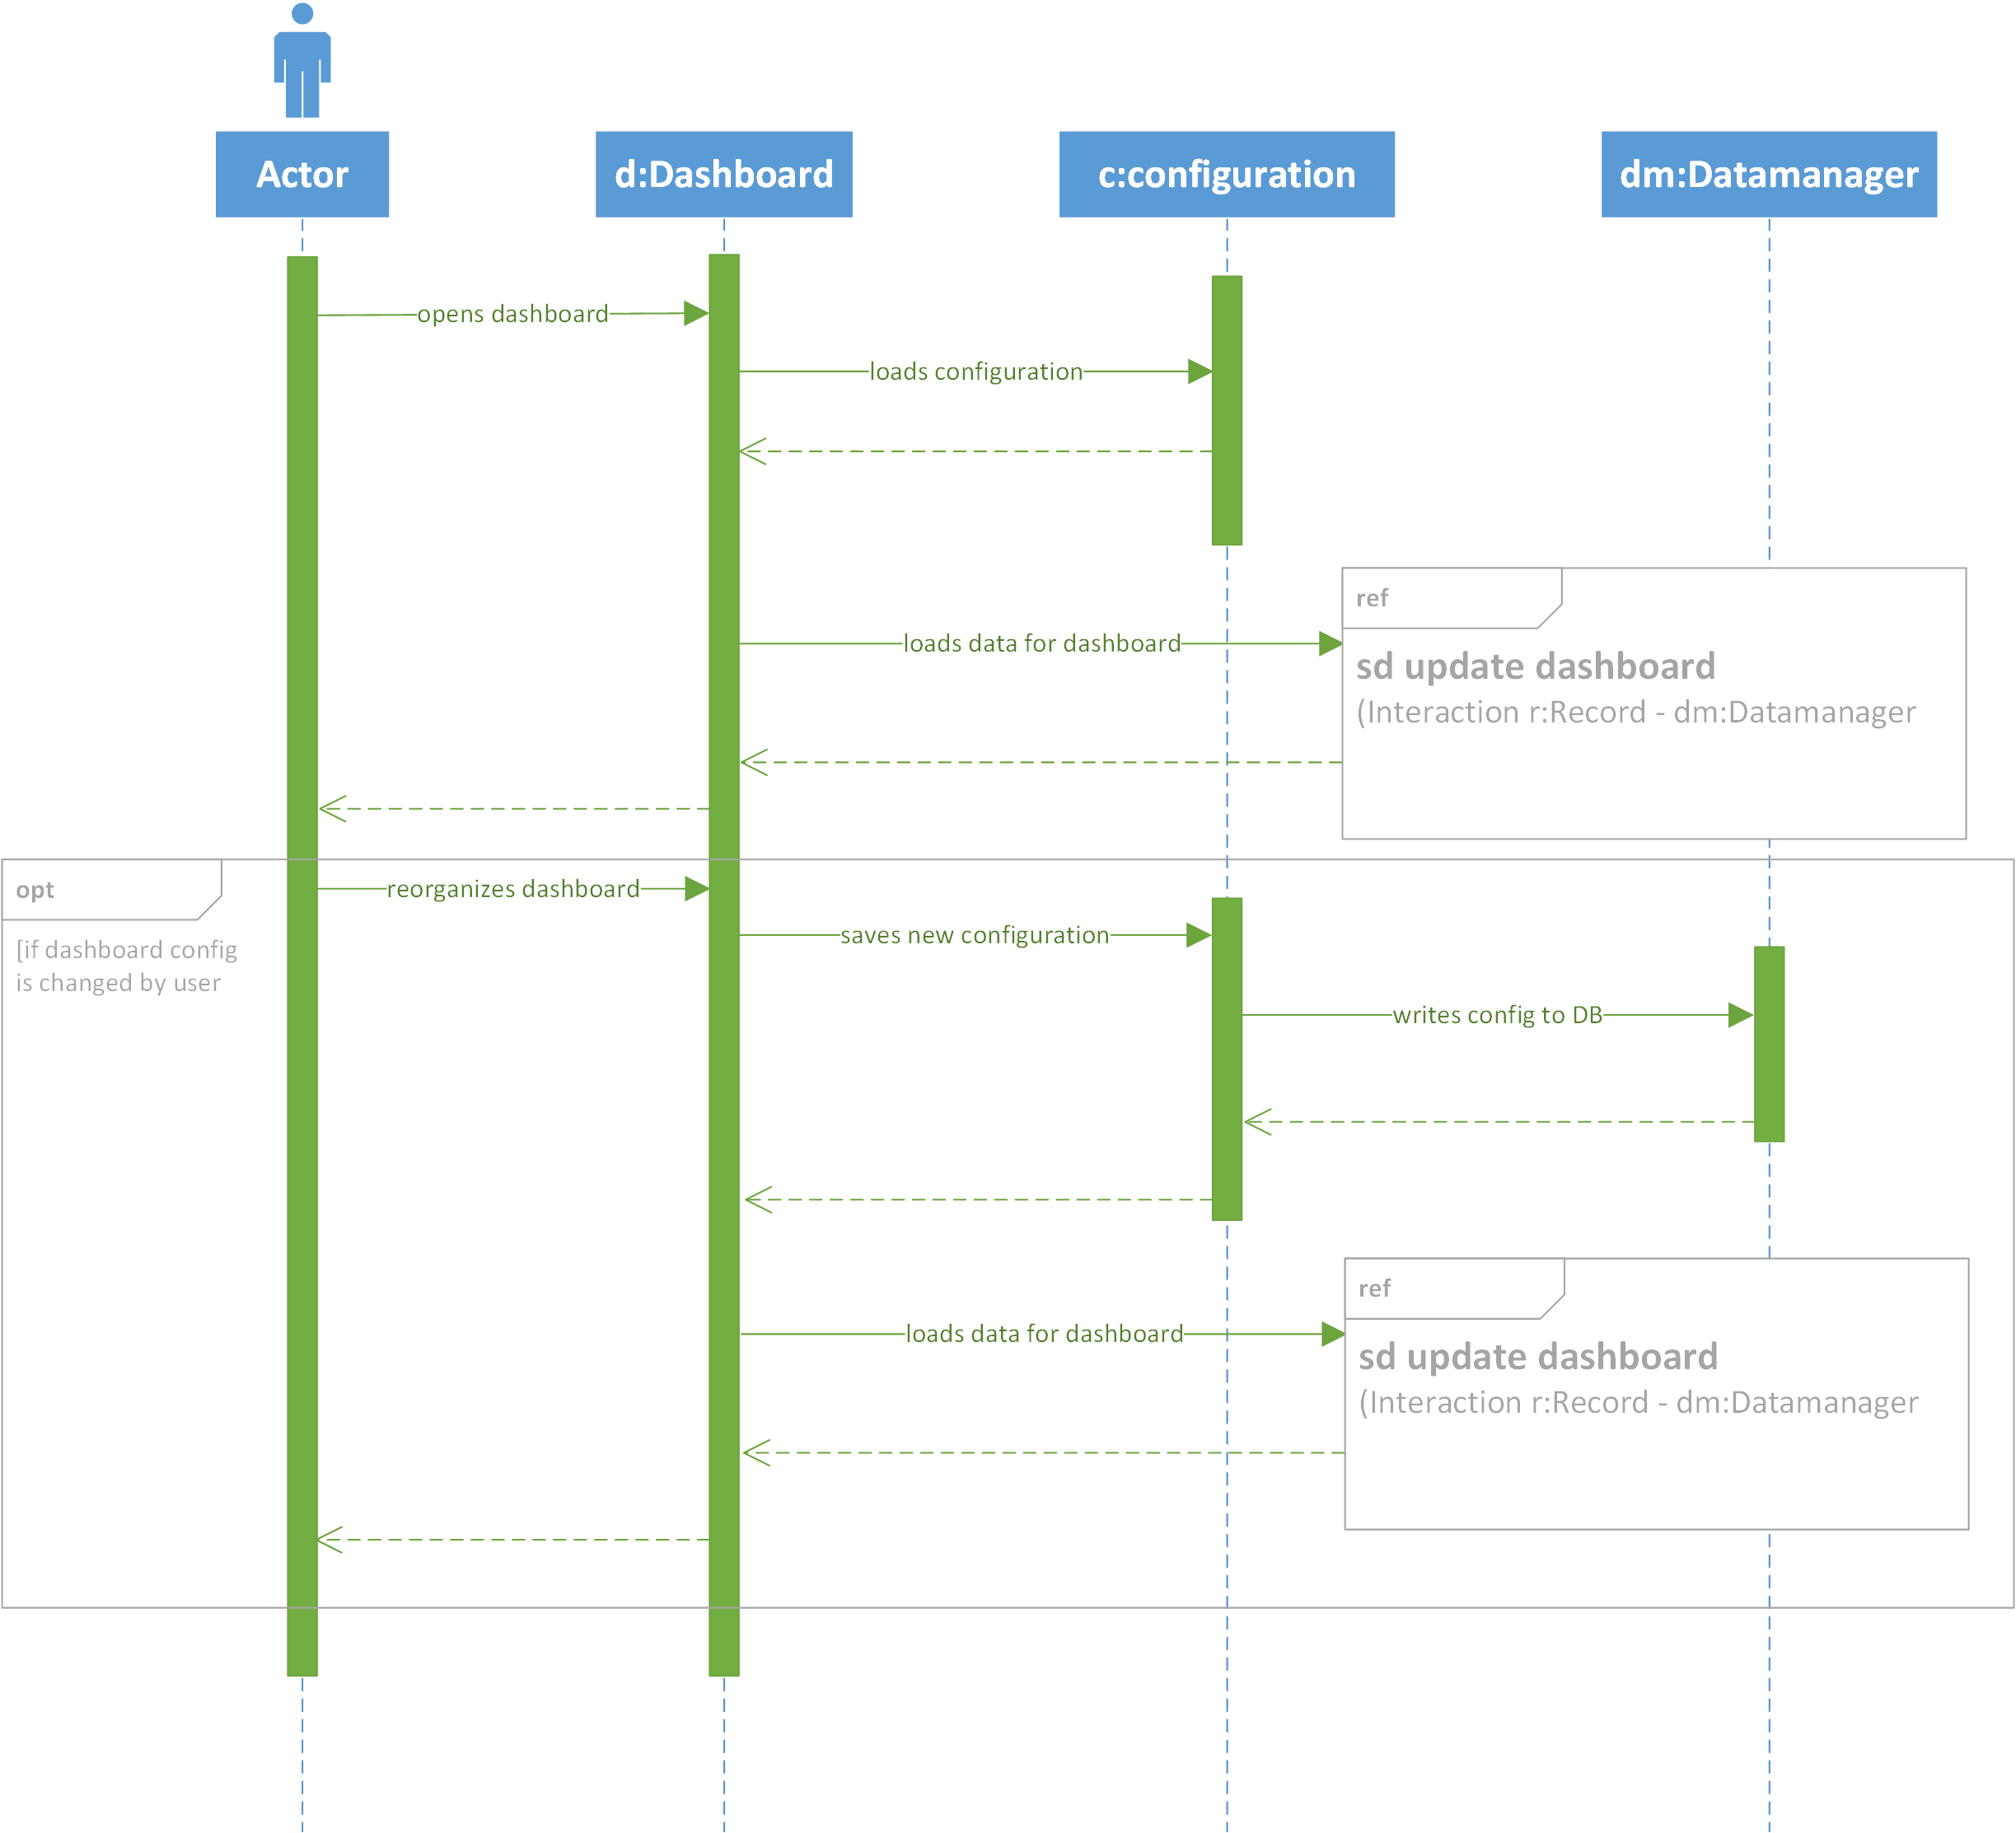
\includegraphics[width=1\textwidth]{./sequence_update.png}

\section{System benachrichtigt Benutzer}
Die mobile Webapplikation prüft nicht automatisch ob neue Daten vorhanden sind. Dies geschieht aber beim Starten der Applikation oder beim neu Laden des Dashboards.
Die Daten werden über einen \textit{Datamanager} bereitgestellt. Dieses Backend analysiert keine Daten, es stellt sie lediglich bereit. Vom Benutzer gesetzte Schwellwerte auf bestimmten Kennzahlen sind dem Datamanager nicht bekannt.

\bigskip

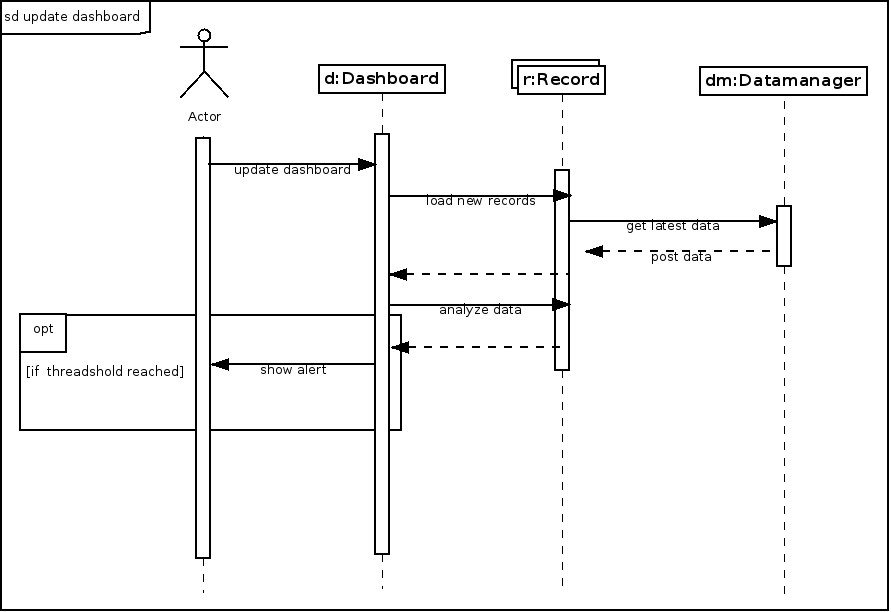
\includegraphics[width=1\textwidth]{./sequence_alert.png}



\end{document}